\documentclass[main.tex]{subfiles}
\begin{document}

For test generation, the ModelTestRelax(MTR,  Version: 3.5.16) framework \cite{mtr} was used with different parameters.

\subsection{Random Walk}
The \textit{Random Walk} algorithm generates a test sequence by randomly selecting a transition from the current state at each step. This process continues until one of the specified stop conditions is met. The algorithm supports two stop conditions:
\begin{itemize}
    \item A given percentage of states has been visited.
    \item A given percentage of transitions has been covered.
\end{itemize}

While \textit{Random Walk} is useful for exploratory testing, it is less efficient for systematic functional testing of large models due to its potentially long test sequences. However, its randomness makes it suitable for uncovering unexpected behaviors.

\subsubsection{Execution and Parameters}
The algorithm is executed using the following parameters:
\begin{itemize}
    \item Coverage type: States or transitions.
    \item Coverage percentage: Desired percentage of coverage.
    \item Reset transitions: Optionally include reset transitions in coverage calculations.
\end{itemize}

\subsubsection{Results}
For this analysis, \textit{Random Walk} was run with 100\% state and transition coverage and also with 75\% state and transition coverage as the stop condition. The last one was repeated five times to account for variability in sequence length and coverage.

\textbf{Results:} After running the Random walk(75\% transition coverage) 5 times, the following statistics can be made.
\begin{table}[H]
\centering
\begin{tabular}{|c|c|c|c|c|}
\hline
 & \textbf{Test Generation Time} & \textbf{Test Sequence Length} & \textbf{Reached coverage} \\ \hline
1 & 0.001434 s & 264 & 77.42\% \\ \hline
2 & 0.000823 s & 41 & 80\% \\ \hline
3 & 0.0008907 s & 58 & 77.42\% \\ \hline
4 & 0.0010825 s & 75 & 77.42\% \\ \hline
5 & 0.0008158 s & 88 & 77.42\% \\ \hline
\textbf{Average} & \textbf{0,0010092 s} & \textbf{105} & \textbf{77.94\%} \\ \hline
\end{tabular}
\caption{Summary of Random Walk Algorithm (5 Runs)}
\label{table:random_walk_summary}
\end{table}
Here we can see that there was one case (namely the first one) where it took much longer time and test sequence to reach the desired coverage or exceed it, which was 77.42\%. This value then was coming up 4 out of 5 times overall. The outstanding long first run is not that surprising since it is a randomized algorithm, if it "chooses worng" multiple times, it will finish later.

\subsection{Transition Tour}

The \textit{Transition Tour} (TT) algorithm is designed to generate the shortest possible test sequence that ensures every transition in a reduced, deterministic, and strongly connected FSM is visited at least once, and returning to the initial state. This approach guarantees full state and transition coverage, making it particularly effective for detecting output faults, though it may not uncover all transfer faults.

The process involves two main stages: 
\begin{enumerate} 
\item Graph Adjustment: The FSM graph is transformed into an Eulerian graph by duplicating certain transitions to balance the number of incoming and outgoing arcs for each state. This step relies on solving a minimum matching problem in a bipartite graph. 
\item Eulerian Path Construction: Using the augmented graph, an Eulerian path is determined by creating a spanning tree where edges point back toward the initial state. 
\end{enumerate}

With a time complexity of $O(n^3 + m)$ and test sequence length proportional to the number of transitions ($O(m)$), the TT algorithm offers an efficient solution for achieving comprehensive coverage in FSM-based testing.

The following figure is an example run on the FSM model.
\begin{figure}[H]
    \centering
    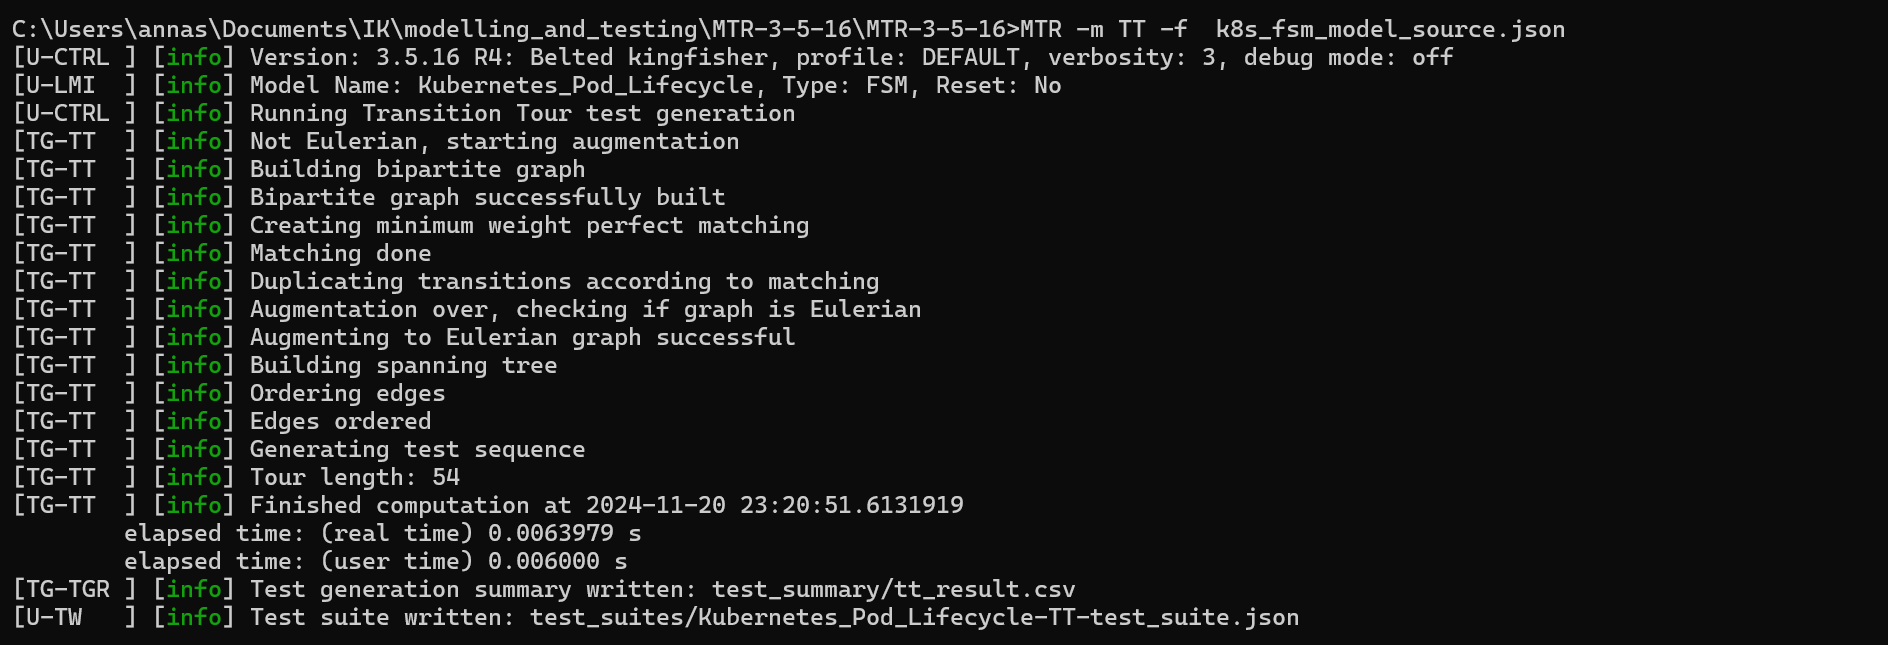
\includegraphics[width=\textwidth]{test_results/TT.png}
    \caption{All-state}
    \label{fig:all_state}
\end{figure}

\subsection{All-State}
The \textit{All-State} algorithm aims to visit every state in the FSM at least once. Using the Nearest Neighbor heuristic, it constructs a test sequence by repeatedly selecting the shortest path to an unvisited state until all states are covered. 

\textbf{Key Characteristics:}
\begin{itemize}
    \item Guarantees 100\% state coverage, but not transition coverage.
    \item Time complexity: $O(n^2)$, where $n$ is the number of states.
    \item Sequence length: $O(m)$, where $m$ is the number of transitions.
\end{itemize}

\subsubsection{Execution and Parameters}
No additional parameters are required for FSMs, but the \texttt{--consider\_reset\_transitions} flag can be used for including reset transitions.
The following figure is an example run on the FSM model.
\begin{figure}[H]
    \centering
    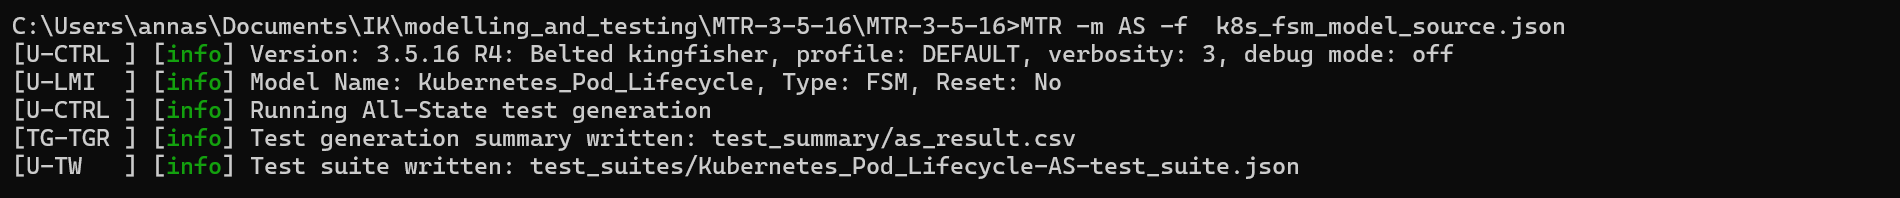
\includegraphics[width=\textwidth]{test_results/AS.png}
    \caption{All-state}
    \label{fig:all_state}
\end{figure}

\subsection{All-Transition-State (ATS)}
\subsubsection{Algorithm Overview}
The \textit{All-Transition-State} (ATS) algorithm generates a test suite that meets two criteria:
\begin{enumerate}
    \item Each transition must be included in a sequence that reaches all FSM states.
    \item Each state must be reachable without using a specific transition (if feasible).
\end{enumerate}

The algorithm operates in two parts:
\begin{itemize}
    \item Preamble: Covers all transitions using the \textit{Transition Tour} method.
    \item Postamble: Covers all states using the Nearest Neighbor heuristic.
\end{itemize}

ATS has three variations:
\begin{itemize}
    \item ATS0: Standard version.
    \item ATSa: Iterative version with no limit.
    \item ATSx: Iterative version with a specified limit.
\end{itemize}

\textbf{Key Characteristics:}
\begin{itemize}
    \item Time complexity: $O(n^3 + m)$ for ATS0; higher for iterative versions.
    \item Sequence length: Comparable to \textit{Transition Tour}.
\end{itemize}

\subsubsection{Execution and Parameters}
For this analysis, the standard version (ATS0) is used.

\subsection{N-Switch Coverage}
The \textit{N-Switch Coverage} algorithm generates test sequences that cover all consecutive $N+1$ transitions in the FSM. It constructs a list of all such paths, selects uncovered paths, and augments sequences as needed to achieve full coverage.

\textbf{Key Characteristics:}
\begin{itemize}
    \item Higher $N$ values increase fault coverage but also lengthen test sequences.
    \item Time complexity: $O((N+1) \cdot m^{N+1})$.
    \item Sequence length: $O((N+1) \cdot m^{N+1})$.
\end{itemize}

\subsubsection{Execution and Parameters}
For this analysis, 1-switch coverage is used as the default configuration.
\begin{figure}[H]
    \centering
    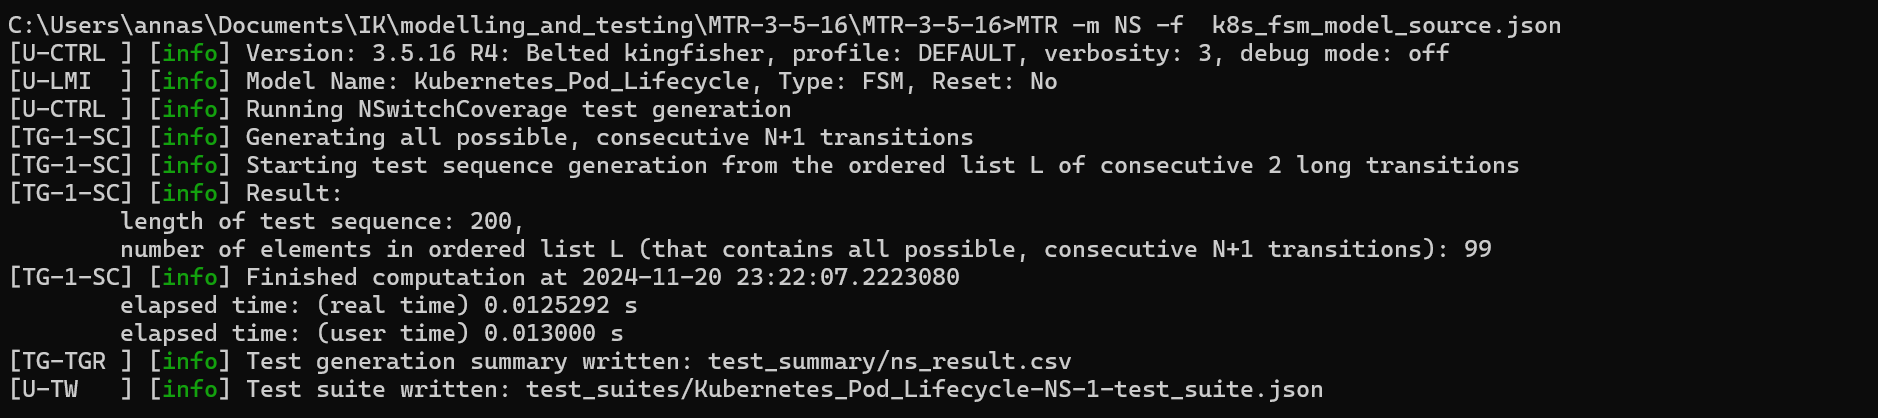
\includegraphics[width=\textwidth]{test_results/n-switch.png}
    \caption{All-state}
    \label{fig:all_state}
\end{figure}

\subsection{Comparison of Test Generation Algorithms}

Table~\ref{tab:algorithm_comparison} summarizes the performance of the selected algorithms based on the FSM model of Kubernetes pod lifecycle management.

\begin{table}[H]
\centering
\caption{Comparison of Test Generation Algorithms}
\label{tab:algorithm_comparison}
\begin{tabular}{|l|c|c|c|}
\hline
\textbf{Algorithm}     & \textbf{Test Sequence Length}     & \textbf{Elapsed Time}      & \textbf{Coverage} \\ \hline
Random Walk (100\% transition c.)     & 965     & 0.0052706 s    & 100\% transition coverage  \\ \hline
All-State     & 18     & 0,0001648 s    & 100\% state coverage \\ \hline
Transition Tour     & 54     & 0.0063979 s  & 100\% state- and transition coverage    \\ \hline
All-Transition-State     & 193     & 0.0244396 s     & 100\% state- and transition coverage    \\ \hline
N-Switch Coverage (N=1)     & 200     & 0.0125292 s     & 100\% state- and transition coverage    \\ \hline
\end{tabular}
\end{table}

\subsection{Conclusions}
The Random Walk (100\% transition coverage) algorithm generated the longest test sequence, consisting of 965 steps, with a moderate elapsed time of 0.00527 seconds, emphasizing complete transition coverage but at the cost of producing lengthy sequences. In contrast, the All-State algorithm created the shortest test sequence of only 18 steps and was the fastest, with an execution time of 0.000165 seconds, as it focuses solely on state coverage, resulting in minimal generation. The Transition Tour algorithm generated a moderate sequence of 54 steps but took slightly longer, with an elapsed time of 0.00640 seconds, reflecting its method of traversing transitions optimally to ensure coverage. The All-Transition-State (ATS) algorithm achieved comprehensive state and transition coverage, producing a sequence of 193 steps but with the highest elapsed time of 0.02444 seconds due to its detailed coverage requirements. Lastly, the N-Switch Coverage (N=1) algorithm provided a balance, generating a sequence of 200 steps with a reasonable elapsed time of 0.01253 seconds, focusing on transitions within a specified depth. These results demonstrate a clear trade-off between coverage, sequence length and execution time.


The generated test suites and result can be found in the github repository: \url{https://github.com/annasz11/kubernetes-mbt}.


\end{document}